%
% firmware.tex
%
% Copyright The TTC 2.0 Contributors.
%
% TTC 2.0 Documentation
%
% This work is licensed under the Creative Commons Attribution-ShareAlike 4.0
% International License. To view a copy of this license,
% visit http://creativecommons.org/licenses/by-sa/4.0/.
%

%
% \brief Firmware project chapter.
%
% \author Gabriel Mariano Marcelino <gabriel.mm8@gmail.com>
%
% \version 0.2.0
%
% \date 2021/05/12
%

\chapter{Firmware} \label{ch:firmware}

.

\section{Product tree}

The product tree of the firmware part of the TTC 2.0 module is available in \autoref{fig:product-tree-fw}.

\begin{figure}[!ht]
    \begin{center}
        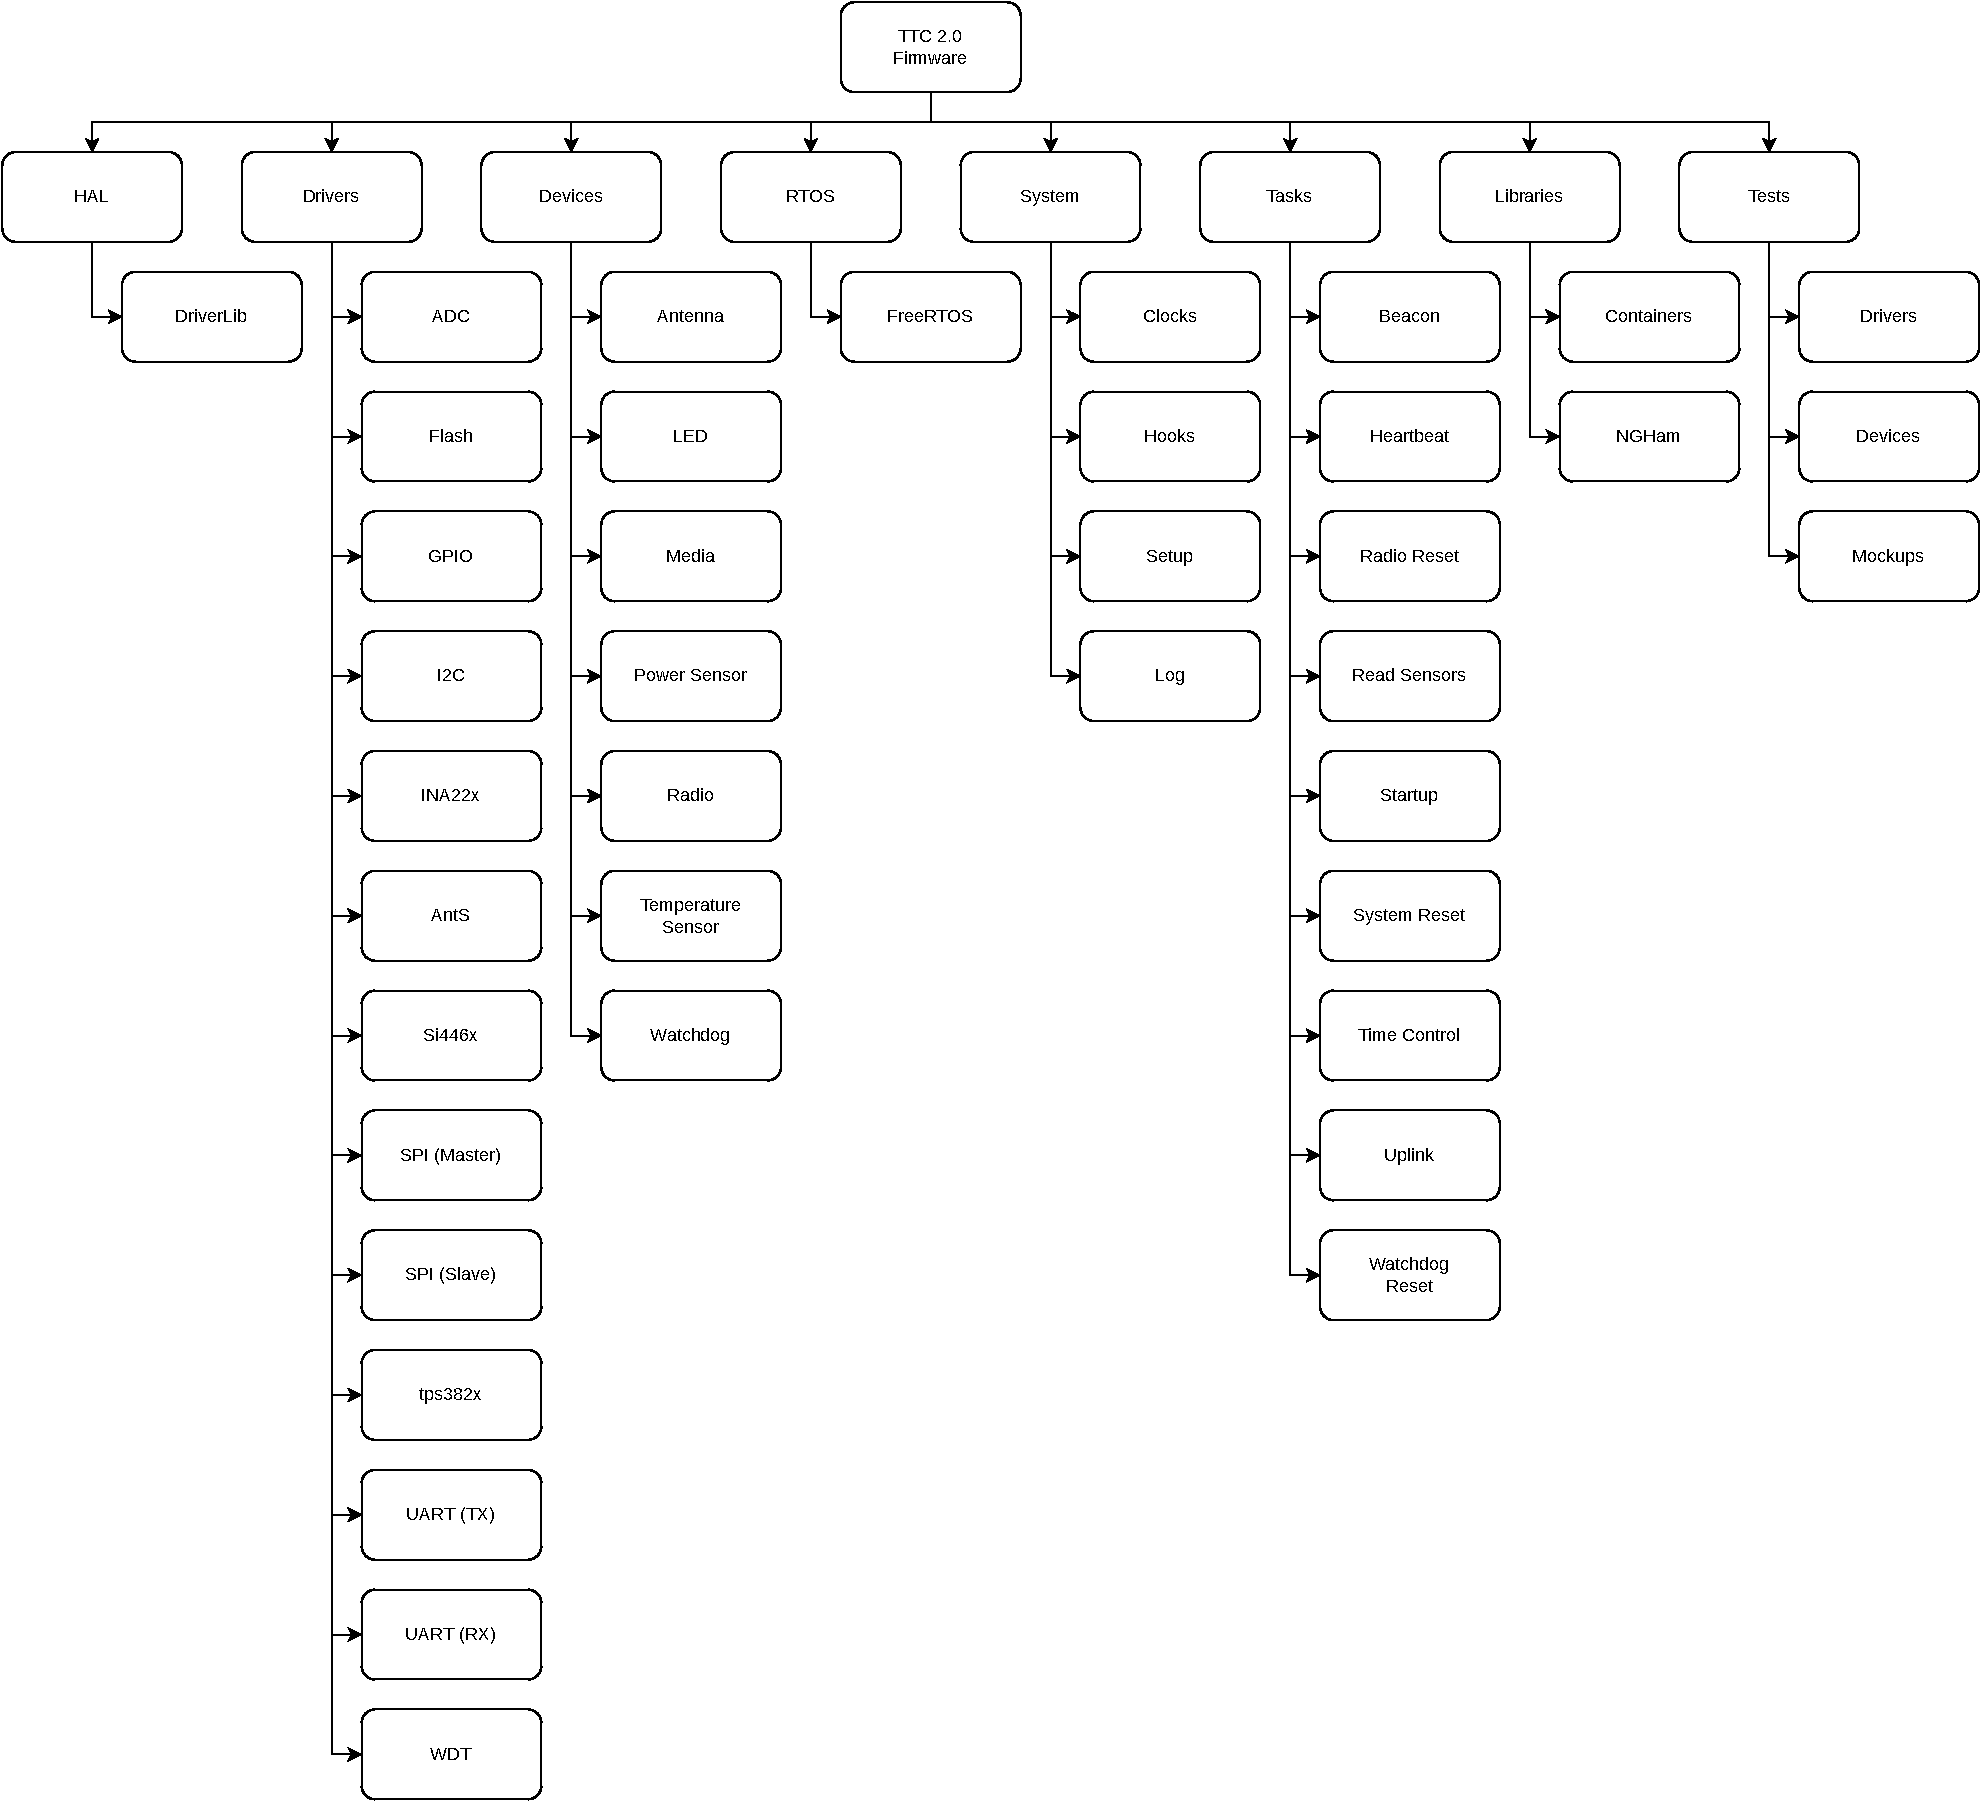
\includegraphics[width=\textwidth]{figures/product-tree-fw.pdf}
        \caption{Product tree of the firmware of the TTC 2.0 module.}
        \label{fig:product-tree-fw}
    \end{center}
\end{figure}

\section{Commands}

The SPI\nomenclature{\textbf{SPI}}{\textit{Serial Peripheral Interface.}} commands of the TTC module are available in \autoref{tab:commands}. All commands are composed by an ID field (1 byte), the content of the command and a checksum at the end of the command (2 bytes). The used checksum algorithm is the CRC16-CCITT\nomenclature{\textbf{CRC}}{\textit{Cyclic Redundancy Check.}} \nomenclature{\textbf{CCITT}}{\textit{Comité Consultatif International Téléphonique et Télégraphique.}} (initial value = 0x0000, polynomial = 0x1021) the value is calculated with the entire packet (ID field + command content).

\begin{table}[!h]
    \centering
    \begin{tabular}{cll}
        \toprule[1.5pt]
        \textbf{ID} & \textbf{Name/Description} & \textbf{Content}\\
        \midrule
        0   & NOP                       & None \\
        1   & Read parameter/variable   & Parameter ID (1B) + Value (4B) + Checksum (2B) \\
        2   & Write parameter/variable  & Parameter ID (1B) + Value (4B) + Checksum (2B) \\
        3   & Transmit packet           & Packet data (1-220B) + Checksum (2B) \\
        4   & Receive packet            & Packet data (1-220B) + Checksum (2B) \\
        \bottomrule[1.5pt]
    \end{tabular}
    \caption{List of commands.}
    \label{tab:commands}
\end{table}

\subsection{Variables and Parameters}

A list of all the variables of TTC with their identification number (ID) and variable type that can be read from the sensors and peripherals is seen in the \autoref{tab:ttc2-variables}.

\begin{longtable}[c]{cL{0.72\textwidth}lc}
    \toprule[1.5pt]
    \textbf{ID} & \textbf{Name/Description} & \textbf{Type} & \textbf{Access} \\
    \midrule
    0   & Device ID (0xCC2A or 0xCC2B)                                      & uint16 & R \\
    1   & Hardware version                                                  & uint8  & R \\
    2   & Firmware version (ex.: ``v1.2.3''' = 0x00010203)                  & uint32 & R \\
    3   & Time counter in millseconds                                       & uint32 & R \\
    4   & Reset counter                                                     & uint16 & R \\
    \multirow{18}{*}{5} & Last reset cause: & \multirow{18}{*}{uint8} & \multirow{18}{*}{R} \\
        & - 0x00 = No interrupt pending                                     &        &  \\
        & - 0x02 = Brownout (BOR)                                           &        &  \\
        & - 0x04 = RST/NMI (BOR)                                            &        &  \\
        & - 0x06 = PMMSWBOR (BOR)                                           &        &  \\
        & - 0x08 = Wakeup from LPMx.5 (BOR)                                 &        &  \\
        & - 0x0A = Security violation (BOR)                                 &        &  \\
        & - 0x0C = SVSL (POR)                                               &        &  \\
        & - 0x0E = SVSH (POR)                                               &        &  \\
        & - 0x10 = SVML\_OVP (POR)                                          &        &  \\
        & - 0x12 = SVMH\_OVP (POR)                                          &        &  \\
        & - 0x14 = PMMSWPOR (POR)                                           &        &  \\
        & - 0x16 = WDT time out (PUC)                                       &        &  \\
        & - 0x18 = WDT password violation (PUC)                             &        &  \\
        & - 0x1A = Flash password violation (PUC)                           &        &  \\
        & - 0x1C = Reserved                                                 &        &  \\
        & - 0x1E = PERF peripheral/configuration area fetch (PUC)           &        &  \\
        & - 0x20 = PMM password violation (PUC)                             &        &  \\
        & - 0x22 to 0x3E = Reserved                                         &        &  \\
    6   & Input voltage of the $\mu$C in mV                                 & uint16 & R \\
    7   & Input current of the $\mu$C in mA                                 & uint16 & R \\
    8   & Temperature of the $\mu$C in K                                    & uint16 & R \\
    9   & Input voltage of the radio in mV                                  & uint16 & R \\
    10  & Input current of the radio in mA                                  & uint16 & R \\
    11  & Temperature of the radio in K                                     & uint16 & R \\
    12  & Last valid command (uplink packet ID)                             & uint8  & R \\
    13  & RSSI of the last valid telecommand                                & uint16 & R \\
    14  & Temperature of the antenna module in K                            & uint16 & R \\
    \multirow{17}{*}{15} & Antenna module status bits:                      & \multirow{17}{*}{uint16} & \multirow{17}{*}{R} \\
        & - Bit 15: The antenna 1 is deployed (0) or not (1)                &        &   \\
        & - Bit 14: Cause of the latest activation stop for antenna 1       &        &   \\
        & - Bit 13: The antenna 1 deployment is active (1) or not (0)       &        &   \\
        & - Bit 11: The antenna 2 is deployed (0) or not (1)                &        &   \\
        & - Bit 10: Cause of the latest activation stop for antenna 2       &        &   \\
        & - Bit 9: The antenna 2 deployment is active (1) or not (0)        &        &   \\
        & - Bit 8: The antenna is ignoring the deployment switches (1) or not (0) &  &   \\
        & - Bit 7: The antenna 3 is deployed (0) or not (1)                 &        &   \\
        & - Bit 6: Cause of the latest activation stop for antenna 3        &        &   \\
        & - Bit 5: The antenna 3 deployment is active (1) or not (0)        &        &   \\
        & - Bit 4: The antenna system independent burn is active (1) or not (0) &    &   \\
        & - Bit 3: The antenna 4 is deployed (0) or not (1)                 &        &   \\
        & - Bit 2: Cause of the latest activation stop for antenna 4        &        &   \\
        & - Bit 1: The antenna 4 deployment is active (1) or not (0)        &        &   \\
        & - Bit 0: The antenna system is armed (1) or not (0)               &        &   \\
    16  & Antenna deployment status (0=never executed, 1=executed)          & uint8  & R \\
    17  & Antenna deployment hibernation (0=never executed, 1=executed)     & uint8  & R \\
    18  & TX enable (0=off, 1=on)                                           & uint8  & R/W \\
    19  & TX packet counter                                                 & uint32 & R \\
    20  & RX packet counter (valid packets)                                 & uint32 & R \\
    21  & TX packets available in the FIFO buffer                           & uint8  & R \\
    22  & RX packets available in the FIFO buffer                           & uint8  & R \\
    23  & Number of bytes of the first available packet in the RX buffer    & uint16 & R \\
    \bottomrule[1.5pt]
    \caption{Variables and parameters of the TTC 2.0.}
    \label{tab:ttc2-variables}
\end{longtable}
